\documentclass[conference]{IEEEtran}
\usepackage{cite}
\usepackage{amsmath,amssymb}
\usepackage{graphicx}
\usepackage{listings}
\usepackage{xcolor}
\usepackage{hyperref}
\usepackage{algorithm}
\usepackage[noend]{algpseudocode}
\usepackage{caption}
\usepackage{subcaption}
\usepackage{tcolorbox}
\usepackage{float}

\title{Multi-Modal Large Language Models for Automated Food and Beverage Label Verification}

\author{
    \IEEEauthorblockN{Lennox Crowe}
    \IEEEauthorblockA{
        \textit{Victoria University of Wellington}
    }
}

\begin{document}
\maketitle

\section{Introduction}
Mislabelling of food products is a persistent cause of food recall events in New Zealand. In 2024, there were 11 consumer-level food recalls initiated due to the presence of undeclared or incorrectly declared allergens after they were packaged or labelled incorrectly~\cite{mpi2024}.

This is not only a safety concern but also has economic repercussions. According to the New Zealand Food \& Grocery Council, the costs of all recalls in New Zealand would be “in the millions of dollars a year”~\cite{fgc2025}.

Manual checks of label correctness are commonplace within the manufacturing industry. Hazard Analysis Critical Control Point (HACCP) is a systematic approach to food safety management~\cite{fda2022}. It is recommended that businesses check label correctness before use in a production area~\cite{mentor2025}. As most manufacturing facilities outsource label printing to suppliers, label rolls may be spliced incorrectly, causing incorrect labels to be applied mid-roll. Frequent manual checks to mitigate this risk are expensive and subject to human error.

Recent advancements in multi-modal LLMs may automate the label checking process, improving timeliness and accuracy.

\section{Related Work}
Many manufacturers will have computer vision systems in place to monitor for defects, orientation, tamper-proof safety seal, and bar-code reading \cite{cognex2025}. In the context of label verification, typically these systems assess the pixel-level difference from one image to the next, rather than the semantic correctness of the printed information.

Optical Character Recognition (OCR) has been used to extract printed information such as expiration dates and part numbers \cite{keyence2025}, but is only sufficiently accurate when extracting a few characters, with predictable styling and positioning. OCR must be combined with Natural Language Processing (NLP) to verify large bodies of text, as small random perturbations will almost always result in OCR errors. 

Currently, OCR and image matching solutions require vendor-specific hardware, often with multiple cameras and dedicated lighting. This introduces strong vendor lock-in and limits what purchased camera equipment can be used for. \cite{cognex2025,keyence2025,antares2025}. 

Recent work has explored multimodal Large Language Models (LLMs), combining computer vision, OCR, and NLP for advanced document understanding. Systems such as QWEN2.5-VL \cite{qwen2_5} and Gemma 3 \cite{gemma3} demonstrate the ability to extract information from images without explicit OCR pipelines. These systems interpret natural language queries, allowing for flexible and intuitive interaction. Despite these developments, limited attention has been given to domain-specific, safety-critical applications such as food and beverage labelling.

\section{System Design}
A mismatch in label layout may not result in a recall, but incorrect critical information (e.g., allergens, contents) can have serious consequences. Traditional approaches to label verification rely on image-matching, which can be sensitive to noise, distortion, and motion blur. Instead, our approach focuses on information-level validation.

The process of verifying label correctness is outlined in the following pseudocode:

\begin{algorithm}
\caption{Label Verification Process}
\begin{algorithmic}[1]
\Function{checkLabel}{label, ground\_truth} \Comment{Returns Boolean}
    \State label\_characteristics $\gets$ \Call{extract}{label}
    \If{label\_characteristics $==$ ground\_truth}
        \State \Return True
    \Else
        \State \Return False
    \EndIf
\EndFunction
\Statex
\State truth $\gets$ \Call{getCorrectLabel}{}
\ForAll{label \textbf{in} production\_line}
    \If{\textbf{not} \Call{checkLabel}{label, truth}}
        \State \Call{stopProduction}{}
    \EndIf
\EndFor
\end{algorithmic}
\end{algorithm}

Three primary components are required:

\begin{enumerate}
    \item \textit{Label Information Extraction (AI Task):}\\
    This step extracts label semantic information, e.g., product name, batch number. These will be extracted by a deep learning model, capable of OCR, NLP, and visual reasoning.
    \item \textit{Ground Truth Reference (Integration Task):}\\
    Each label must be compared against a reference. Most manufacturers have a database mapping stock keeping unit (SKU) codes to label images or metadata. These references can be processed using the same extraction model to ensure format consistency.
    \item \textit{Label Comparison Logic (Software Engineering Task):}\\
    After building semantic representations of the label and the reference, these are compared to form a boolean output: either the label matches the reference or it does not. Label semantic information can be stored in a dictionary of name-value pairs. For example:

\begin{verbatim}
{
    sku: AB1234, 
    contents: 60 capsules, 
    vitamins: [D3, K2], 
    batch: Z987
}
\end{verbatim}

This is akin to a question-answering task:

\begin{itemize}
  \item What is the SKU number?
  \item What are the contents?
  \item What vitamins are listed?
  \item What is the batch number?
\end{itemize}

If any answer differs from the ground truth, the label is incorrect:
\begin{verbatim}
truth:      {contents: 60 capsules}
comparison: {contents: 120 capsules}
\end{verbatim}
\end{enumerate}

\section{Expected Results}
The most technically challenging component is Task 1: label information extraction using deep learning. Tasks 2 and 3 primarily involve software integration and logic.

This task falls under OCR-VQA (Optical Character Recognition for Visual Question Answering), where the model answers domain-specific questions based on image content. Models such as QWEN2.5-VL and Gemma3 \cite{qwen2_5} \cite{gemma3} show promising performance at OCR-VQA tasks. This project will focus on fine-tuning pretrained models to achieve high accuracy on domain specific label information extraction tasks.

Overall, label verification is a binary classification task: labels either match the reference or not. However, the chosen OCR-VQA model is concerned with providing accurate semantic representations of the label. Accurate semantic representations will lead to high precision and recall in the binary classification task. The primary evaluation metric for the AI model will be accuracy of semantic information, i.e. the proportion of key-value pairs which are correct. An extra consideration is inference speed. To be used in a manufacturing facility, the model must have quick inference time. Low parameter models should be investigated for a tradeoff of accuracy to inference speed.

A full deployment would integrate the model into a live production environment (via API/UI) for real-time monitoring at a manufacturing facility. While full implementation is beyond the scope of this project, a demonstration ready API is required to perform label-verification.

\section{Proof of Concept}

To assess feasibility, a proof-of-concept was conducted using the open source QWEN2.5-VL pre-trained model on a small set of label images. The goal was not to comprehensively evaluate performance, but rather to observe if existing models can already extract semantic information from labels.

Our early experiments showed that semantic information could be extracted with reasonable accuracy, but fine-tuning will be necessary for good performance. An example image, prompt, and output is shown in Fig.~\ref{fig:poc}.

\begin{figure}[H]
    \centering
    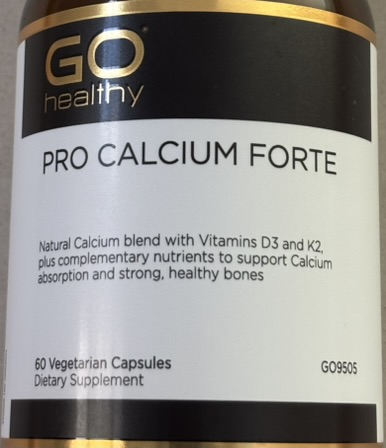
\includegraphics[width=0.4\linewidth]{label5.JPEG}
    \caption*{\footnotesize Image of a dietary supplement label}

    \textbf{Prompt:}
    \begin{lstlisting}[basicstyle=\ttfamily\scriptsize, frame=single, breaklines=true]
This is an image of a vitamin supplement label. Use the text in the image to extract the following information: SKU number, name of the product, contents (number of capsules), and a list of contained vitamins. Output in the following JSON format: {"sku": "<SKU NUMBER>", "product_name": "<PRODUCT_NAME>", "contents": "<CAPSULES_NUMBER>", "vitamins": ["<VITAMINS_1>", ..., "<VITAMINS_N>"]}
    \end{lstlisting}

    \textbf{Model Output:}
    \begin{lstlisting}[basicstyle=\ttfamily\scriptsize, frame=single, breaklines=true]
{
  "sku": "GO9505",
  "product_name": "PRO CALCIUM FORTE",
  "contents": "60 Vegetarian Capsules",
  "vitamins": ["D3", "K2"]
}
    \end{lstlisting}

    \caption{Proof-of-concept using QWEN2.5-VL to extract structured label data}
    \label{fig:poc}
\end{figure}

\section{System Resources and Development Environment}

\subsection{Hardware}
Initial development and testing with small models and datasets will be carried out on a local workstation equipped with a NVIDIA RTX 3060 GPU (12~GB VRAM). For training larger models, the project will leverage university-provided GPU servers, which include high memory configurations of up to 48~GB VRAM per GPU. This approach enables efficient development while accommodating the resource demands of training large models.

\subsection{Software}
The system will be implemented in Python, using open source deep learning frameworks such as PyTorch. For transfer learning tasks, Hugging Face Transformers will be loaded into a suitable deep learning framework, and then fine-tuned.

\section{Conclusion}

Advances in multi-modal LLMs offer opportunity to automate food and beverage label verification, with semantic understanding comparable to human inspection. A model that balances accuracy and inference speed could enable practical, cost-effective deployment in manufacturing facilities worldwide.

\section{Statement}

This report and all related work is solely my own. Tools used include LaTeX, git, Python 3.12, Pytorch 2.7.1, and Hugging Face transformers, specifically QWEN 2.5-VL. Code for the proof of concept can be accessed here: https://github.com/LennoxC/qwen2-testing.

\begin{thebibliography}{1}
\bibitem{mpi2024}
Ministry for Primary Industries, \emph{Consumer-level Food Recalls Annual Report 2024}. Wellington: New Zealand Food Safety Food Compliance Services, 2024.

\bibitem{fgc2025}
New Zealand Food \& Grocery Council, “Product Recall Withdrawal,” \emph{fgc.org.nz}, para. 6. [Online]. Available: \url{https://www.fgc.org.nz/product-recall-withdrawal}. [Accessed: Aug. 23, 2025].

\bibitem{fda2022}
U.S. Food and Drug Administration, \emph{Hazard Analysis Critical Control Point (HACCP)}. Maryland: FDA Human Foods Program, 2022.

\bibitem{mentor2025}
“How to verify your food labels,” \emph{haccpmentor.com}, para. 6. [Online]. Available: \url{https://haccpmentor.com/verify-food-labels/}. [Accessed: Aug. 23, 2025].

\bibitem{cognex2025}
“Label Quality Inspection,” \emph{cognex.com}. [Online]. Available: \url{https://www.cognex.com/industries/food-and-beverage/packaging-inspection/label-and-packaging-quality-inspection}. [Accessed: Aug. 23, 2025].

\bibitem{keyence2025}
“OCR Verification and Character Inspection,” \emph{keyence.com}. [Online]. Available: \url{https://www.keyence.com/products/vision/vision-sys/applications/ocr-verification-and-character-inspection.jsp}. [Accessed: Aug. 23, 2025].

\bibitem{antares2025}
“Label Inspection for cylindrical vertical products – IE4000 PLUS,” \emph{antaresvisiongroup.com}. [Online]. Available: \url{https://antaresvisiongroup.com/food/products/label-inspection-for-not-oriented-containers-ie-4000/}. [Accessed: Aug. 23, 2025].

\bibitem{qwen2_5}
Yang, A., Li, A., Yang, B., Zhang, B., Hui, B., Zheng, B., ... & Qiu, Z. (2025). Qwen3 technical report. arXiv preprint arXiv:2505.09388.

\bibitem{gemma3}
Team, G., Kamath, A., Ferret, J., Pathak, S., Vieillard, N., Merhej, R., ... & Iqbal, S. (2025). Gemma 3 technical report. arXiv preprint arXiv:2503.19786.

\end{thebibliography}

\end{document}

